\section{Appendix} \label{sec:appendix}
\subsection{Appendix A: Old Driver Module Design} \label{sec:appendix:old_driver_module_design}

As visible from figure \ref{fig:registerModuleOverview}, the old driver module has two parts: common interface, select interface. Connection to registers is the bridge between the driver module and registers in the register module.

We used two demuxers to create the common interface. The basic idea behind this implementation is the following: DEC pin defines the way where CE and CLK signals are propagated, so DEC is connected to the select pin of both demuxers. CE switches the signals off or on, while CLK stimulates the alterations in UP/DOWN pairs, contributing to the change in the value of a register. 

Because of the inner circuit of 74LS193, we need to avoid simultaneous pulsing and UP/DOWN pair grounded since it unfavorably alters the value of a register. The solution was quite straightforward: CLK pin of the driver module is connected to the output of anded clock signal and CE pin. 

The resulting UP/DOWN pair is directed to the select interface, that redirects the pair to a specific, selected, register. This behavior is accomplished by utilizing 3-to-8 demuxers, because we have less than 8 registers but more than 4.

\begin{figure}[H]
	\centering
	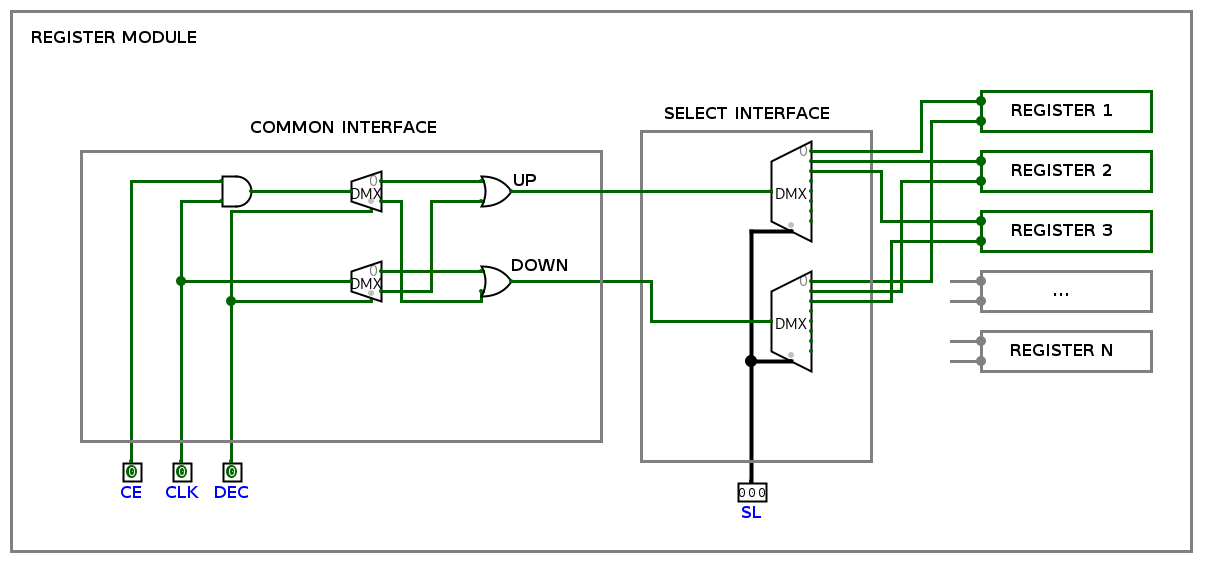
\includegraphics[width=0.9\textwidth]{img/driver_module_implementation}
	\caption{The Old Driver Module Implementation}
	\label{fig:driverModuleImplementation}
\end{figure}